
\chapter{Interest Rates and Bond Models}

Throughout the previous chapter the risk-free interest rate $r$ was a constant --- a convenient fiction, and we knew it.
In reality interest rates fluctuate, driven by central banks and by the market itself, and their dynamics governs the pricing of \emph{bonds}, the most fundamental fixed-income securities and by volume one of the largest markets in the world.
This chapter develops the theory of bond pricing under stochastic interest rates.
The plot will feel familiar: as with options, a hedging argument plus no-arbitrage produces a pricing PDE; but there is a new twist --- the underlying ``asset'', the rate $r$, is not itself tradable --- and resolving it introduces a genuinely new object, the market price of risk.
The chapter culminates in the Vasi\v{c}ek model and its complete solution.
% CLAUDE NOTE (unreviewed PDF): These notes are "mostly good" but unreviewed.
% Original notation is preserved; corrections and expansions are added where needed.


\section{Bond fundamentals}

A \emph{bond} is a debt instrument issued by a state or corporation (the \emph{writer}) to an investor (the \emph{holder}).
The holder lends capital, and in exchange acquires the right (a) to the reimbursement of the capital lent, (b) with an interest, (c) at a future date $T$, the \emph{maturity}.
As with options, the price of the contract must be \emph{fair}, and the task of the chapter is to say what that means quantitatively.

\paragraph*{Constant interest rate.}

We warm up by assuming $r = \text{const.}$, even though $r$ is in general stochastic.
Let $B(t)$ be the value of the bond at time $t$.
Over an infinitesimal step the bond simply accrues interest,
\begin{equation}
B(t)\bigl(1 + r\,dt\bigr) = B(t+dt),
\end{equation}
which is nothing but the cost of money.
In differential form,
\begin{equation}
\frac{B(t+dt) - B(t)}{B(t)} = \frac{dB(t)}{B(t)} = r\,dt
\quad\Longrightarrow\quad
B(T) = B(t)\, e^{r(T-t)},
\end{equation}
the compound-interest law of Section~\ref{sec:bank-account} again.

In the market, bonds are classified by their maturity: \emph{short-term} ($\le 1$ year), \emph{medium-term} (1--5 years), \emph{long-term} (5--10 years), and \emph{very long-term} (10--50 years); holder and writer agree on the maturity at signing.
Depending on the issuer one speaks of \emph{government bonds} --- by far the most widespread and traded --- or \emph{corporate bonds}.
% CLAUDE NOTE: the government/corporate distinction is from the course slides
% (Mercati & Strumenti Finanziari), added 2026-07-06.
For the theory, however, maturity, issuer, and face value are inessential bookkeeping, and it is convenient to normalize them away: for any $T$, any issuer, and any face value we set
\begin{equation}
B(T)=1,
\end{equation}
i.e.\ every bond pays one unit of currency at maturity.
With constant $r$ the problem is then completely solved,
\begin{equation}
B(t) = e^{-r(T-t)}:
\end{equation}
the bond today is worth the discounted unit payment.
Everything that follows is about what survives of this formula when $r$ starts to move.


\section{Stochastic interest rates}\label{sec:stochastic-rates}

The assumption $r = \text{const.}$ is not really tenable.
The rate $r(t)$ is a \emph{spot rate} --- the rate for instantaneous borrowing, quoted now --- and its future values are unknown; by the EMH of the previous chapter, it should itself follow an SDE, $dr(t)$.

Why do rates fluctuate?
The causes are of two kinds, and it is worth keeping them apart.

The first kind is \emph{exogenous} to the market but endogenous to the economy: rates are steered at the table of the central banks (FED, BCE, \ldots) as their principal policy instrument.
Two standard scenarios: when inflation is high, the bank \emph{raises} $r$ to encourage saving over spending; when the economy stagnates, it \emph{lowers} $r$ to stimulate consumption and investment.
The direction of the next intervention may be guessable, but its timing is not --- and every surprise decision instantly modifies the value of all outstanding bonds.

The second kind is \emph{endogenous} to the market, and works in two stages.
Bonds are born on the \emph{primary market}, where the issuer places a certain volume with a face value but no fixed price; only a restricted circle of institutions can participate, through a competitive auction mechanism.\footnote{In Italy, the BOTs (Buoni Ordinari del Tesoro) are placed exactly this way.}
They then move to the \emph{secondary market}, where small banks and individual investors trade them freely --- and there $B(t)$ fluctuates like any other price.

The fluctuations are anything but small.
Figure~\ref{fig:treasury} shows the US 10-Year Treasury constant-maturity rate --- the world's reference ``risk-free'' rate --- which rose from about 4\% in the early 1960s to above 14\% in the inflationary early 1980s, then declined for four decades toward 1--2\% by 2020.
A model with constant $r$ cannot even begin to describe such a history.

% Real-data figure (replaces the chart pasted in the raw notes, page 3);
% generated by images/code_for_images/treasury_10y.py from FRED series GS10.
\begin{figure}[h!]
\centering
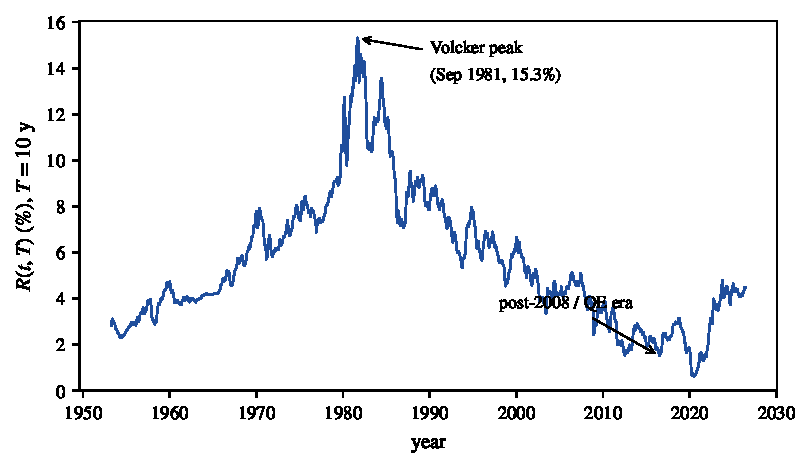
\includegraphics[width=0.9\textwidth]{images/treasury_10y.pdf}
\caption{US 10-Year Treasury constant-maturity yield, monthly averages, 1953--2026. Data: FRED, series GS10 (Federal Reserve Bank of St.\ Louis). Generated by \texttt{images/code\_for\_images/treasury\_10y.py}.}
\label{fig:treasury}
\end{figure}


\section{The yield to maturity and the yield curve}

If the growth rate of a bond is no longer constant, the exponent in $B(T)=B(t)\,e^{r(T-t)}$ must be replaced by an effective, maturity-dependent rate.
One writes
\begin{equation}
B(T) = B(t)\, e^{R(t,T)(T-t)},
\end{equation}
where $R(t,T)$ is the \emph{yield to maturity} (rendimento a scadenza): the constant rate that, applied over $[t,T]$, would reproduce the actual growth of the bond.
It depends on both the present time $t$ and the maturity $T$.
Using the normalization $B(T)=1$ and solving for $R$,
\begin{equation}
B(t) = e^{-R(t,T)(T-t)}
\;\Longrightarrow\;
\ln B(t) = -R(t,T)(T-t)
\;\Longrightarrow\;
R(t,T) = -\frac{1}{T-t}\,\ln B(t).
\end{equation}
So the market prices of bonds determine $R(t,T)$, and plotting it against the maturity $T$ at fixed $t$ produces the \emph{yield curve} (curva dei rendimenti) --- the single most watched graph in fixed income, to which we return in the final section.

From the yield to maturity one recovers the instantaneous rate as the short-maturity limit,
\begin{equation}\label{eq:spot-rate}
r(t) := \lim_{(t-T)\to 0} R(t,T) = \lim_{(t-T)\to 0}\Bigl(-\frac{1}{T-t}\ln B(t)\Bigr),
\end{equation}
which is formally indeterminate --- $B(T)=1$ makes the numerator vanish together with the denominator --- but converges, exactly as a derivative does.
The \emph{spot rate} $r(t)$ is the object our stochastic models will describe.


\section{The Vasi\v{c}ek model for bond pricing}\label{sec:vasicek-model}

The bond pricing model of Vasi\v{c}ek\cite{Vasicek1977} stands to bonds as Black--Scholes stands to options, and we will construct it along the same lines: hypotheses, hedged portfolio, no-arbitrage, PDE.

\paragraph*{Hypotheses.}

\begin{enumerate}[label=(\roman*)]
    \item There is market risk, but no credit risk.
    \item The short rate is assumed to be a Markov It\^o diffusion.
    \item The no-arbitrage principle holds.
    \item The interest rate follows the SDE
    \begin{equation}\label{eq:rate-sde}
    dr(t) = f(r,t)\,dt + S(r,t)\, dW_t,
    \end{equation}
    with drift and diffusion functions $f$ and $S$ to be specified later.
\end{enumerate}
The parallel with the stock case, $dS(t) = \mu S\,dt + \sigma S\,dW_t$, is deliberate, but the analogy must be handled with care: there, the underlying $S$ was a \emph{tradable} asset; here, one cannot buy ``one unit of interest rate''.
The chain of dependence is $r \to dr \to B(r,t;T)$, in parallel with $S \to dS \to O(S,t)$.

Let us compute how a bond price responds to the rate.
Given $B = B(r,t; T)$, It\^o's formula applied along~\eqref{eq:rate-sde} gives
\begin{equation}
dB = \biggl(\frac{\partial B}{\partial t} + f(r,t)\frac{\partial B}{\partial r} + \frac{1}{2}S^2(r,t)\frac{\partial^2 B}{\partial r^2}\biggr)dt + S(r,t)\frac{\partial B}{\partial r}\, dW_t.
\end{equation}
It is convenient to give names to the relative drift and volatility of the bond.\footnote{The notation follows the notes: $\mu$ and $\sigma$ here refer to the bond's return and volatility, not the stock's.}
We define
\begin{align}
\mu(t,T) &= \frac{1}{B(r,t;T)}\biggl(\frac{\partial B}{\partial t} + f(r,t)\frac{\partial B}{\partial r} + \frac{1}{2}S^2(r,t)\frac{\partial^2 B}{\partial r^2}\biggr), \\[4pt]
\sigma(t,T) &= -\frac{1}{B(r,t;T)}\, S(r,t)\,\frac{\partial B}{\partial r} > 0,
\end{align}
so that $\mu(t,T)$ is the instantaneous return of the bond and $\sigma(t,T)$ its volatility.
The minus sign in the definition of $\sigma$ is a sign convention chosen to make $\sigma$ positive, and it encodes a genuine piece of economics: the rate and the bond price are \emph{anticorrelated}.
If $dr > 0$, i.e.\ $r(t+dt) > r(t)$, then $B(r+dr) < B(r)$, so $dB < 0$.
A concrete example: let $T = 1$ year and suppose the BCE raises the annual rate from 2\% to 4\%.
Newly issued bonds now yield 4\%; the old ones, still promising 2\%, are suddenly less attractive, and their market price drops until their effective yield matches.

\subsection{The hedging portfolio}

We now look for the analogue of the delta-hedged portfolio.
There is an immediate obstruction: in Black--Scholes we hedged the option \emph{with the underlying stock}, but here the underlying is $r$, which cannot be held.
The resolution is to hedge \emph{one bond with another}: bonds of different maturities respond to the same $r$, so a suitable combination can be made riskless.

Let $B_i=B(r,t;T_i)$, $\mu_i=\mu(t,T_i)$ and $\sigma_i=\sigma(t,T_i)$.
Choose holdings $h_1,h_2$ and position values $V_i=h_iB_i$ in a self-financing portfolio of value $\Pi=V_2-V_1$.
Then
\[
 d\Pi=h_2\,dB_2-h_1\,dB_1
 =(V_2\mu_2-V_1\mu_1)\,dt-(V_2\sigma_2-V_1\sigma_1)\,dW_t.
\]
The holdings are adjusted so that $V_2\sigma_2=V_1\sigma_1$.
For $\sigma_1\ne\sigma_2$, the value and hedge conditions give
\[
 V_1=\frac{\Pi\sigma_2}{\sigma_1-\sigma_2},\qquad
 V_2=\frac{\Pi\sigma_1}{\sigma_1-\sigma_2}.
\]
Consequently the riskless portfolio satisfies
\[
 d\Pi=\Pi\frac{\mu_2\sigma_1-\mu_1\sigma_2}{\sigma_1-\sigma_2}\,dt=r\Pi\,dt,
\]
and hence
\[
 \sigma_1(\mu_2-r)=\sigma_2(\mu_1-r).
\]
The adjustable quantities are the holdings, not the quoted bond prices.
This is the same self-financing condition used in Chapter~5.

Rearranging so that each maturity keeps to its own side,
\begin{equation}\label{eq:vasicek-identity}
\frac{\mu(t,T_1) - r}{\sigma(t,T_1)} = \frac{\mu(t,T_2) - r}{\sigma(t,T_2)},
\end{equation}
valid $\forall\, t \le \min(T_1, T_2)$ and, crucially, $\forall\, T_1, T_2$.
This is the \textbf{Vasi\v{c}ek identity}, a dynamic identity of the model: the excess return per unit of volatility, $\frac{\mu - r}{\sigma}$, is the \emph{same for all bonds}, whatever their maturity --- a kind of separation of variables, with the maturity dropping out of the ratio.

\paragraph*{The market price of risk.}

Since the ratio in~\eqref{eq:vasicek-identity} does not depend on the maturity, it defines a function of $r$ and $t$ alone.
We give it a name:
\begin{equation}\label{eq:market-price-risk}
q(r,t) := \frac{\mu(r,t;T) - r}{\sigma(r,t;T)},
\end{equation}
the \emph{market price of risk}.
It measures the compensation --- excess return per unit of volatility --- that the market demands for bearing interest-rate risk, i.e.\ the aggregate risk aversion of bond investors.
In Black--Scholes no such object appeared, because hedging with the tradable underlying eliminated the risk premium entirely; here, where $r$ is not tradable, a residue of the market's attitude toward risk survives in the pricing equation.

To obtain that equation, write $q\,\sigma = \mu - r$ and substitute the definitions of $\mu$ and $\sigma$; the terms reassemble into
\begin{equation}\label{eq:term-structure}
\boxed{\frac{\partial B}{\partial t} + \bigl(f + S\,q\bigr)\,\frac{\partial B}{\partial r} + \frac{1}{2}S^2\,\frac{\partial^2 B}{\partial r^2} = r\, B}
\end{equation}
with boundary condition $B(r, t=T; T) = 1$.
This is the \textbf{term structure equation}, the exact analogue of the Black--Scholes equation $\partial_t O(S,t) + \ldots = rO$ for bonds.

Several remarks are in order before we solve it.
First, note the structural difference from Black--Scholes: there the discounting rate $r$ on the right-hand side was a fixed constant, while here the $r$ multiplying $B$ is the fluctuating state variable itself --- the same symbol, two very different roles.
Second, the equation is not yet specified: the functional forms of $f$ and $S$ must be modelled, and GBM will \emph{not} do --- an interest rate does not grow exponentially (if it did, no state could ever afford to issue bonds).
Third, taking $q$ constant is an additional modelling assumption, not a consequence of the ratio defining it.
With the bond convention $dB/B=\mu\,dt-\sigma\,dW$, the Girsanov kernel of Section~\ref{sec:rn-girsanov} is $\varphi=q$.
Thus $dW=q\,dt+dW^Q$ and the short-rate drift under $Q$ is $f+Sq$.
Finally, the Feynman--Kac formula of Chapter~5 offers an alternative representation of the solution,
\begin{equation}
B(r,t;T) = E^Q\!\Bigl[\exp\Bigl\{-\int_t^T r(s)\,ds\Bigr\}\,\Bigm|\,r(t)=r\Bigr],
\end{equation}
a discounted expectation as before --- except that now $r(s)$ is stochastic, so the discount factor sits \emph{inside} the expectation, integrated along each trajectory.
One could evaluate this average directly, but we will follow the PDE route instead.


\section{The Vasi\v{c}ek solution}\label{sec:vasicek-solution}

\subsection{The Ornstein--Uhlenbeck model for the interest rate}

To make the term structure equation concrete we must choose the model
\begin{equation}\label{eq:vasicek-sde}
dr(t) = f(r,t)\, dt + S(r,t)\, dW_t,
\end{equation}
i.e.\ commit to functional forms for $f$ and $S$.
What do we require of a sensible rate model?
That for long times $r$ neither explodes nor collapses, but hovers around a stable level with small fluctuations --- exactly the behaviour of the mean-reverting process we solved in Chapter~4.
Vasi\v{c}ek's choice is indeed the Ornstein--Uhlenbeck process\cite{UhlenbeckOrnstein1930}, shifted to revert to a nonzero level: the (essentially unique, by Doob's theorem) Markov, Gaussian, stationary process.
Its It\^o SDE is
\begin{equation}\label{eq:ou-rate}
dr(t) = \alpha\bigl[\theta - r(t)\bigr]dt + \sigma\, dW_t,
\end{equation}
with $\alpha, \theta, \sigma > 0$ and $[\alpha] = [t]^{-1} = \tau^{-1}$.
Here $\theta$ is the \emph{long-run mean} toward which the rate is pulled, and we note already that $\theta$ is \emph{not} simply the historical mean of the observed time series.\footnote{Under the historical measure, $\theta$ is the long-run mean and can be estimated from sufficiently long rate data.
The pricing parameter is the risk-adjusted mean $\theta^*$ defined below. See Section~\ref{sec:vasicek-calibration}.}

Although the solution parallels Chapter~4, we spell it out, both because the nonzero mean changes the formulas and because the notes' derivation is compact.
% CLAUDE NOTE: The notes' intermediate steps for the variable change are somewhat
% compressed (they write f(r,t) = r e^{αt} and a chain of substitutions x:=E, f(x)=x²=r).
% We present the standard derivation of the OU solution via Doob's transform.
Apply It\^o's lemma to the function $g(r,t) = r\, e^{\alpha t}$, for which $\partial_r g = e^{\alpha t}$ and $\partial_t g = \alpha r\, e^{\alpha t}$:
\begin{equation}
dg(r,t) = \bigl[\alpha r\, e^{\alpha t} + \alpha(\theta - r)\, e^{\alpha t}\bigr]dt + \sigma\, e^{\alpha t}\, dW_t = \alpha\theta\, e^{\alpha t}\, dt + \sigma\, e^{\alpha t}\, dW_t;
\end{equation}
the mean-reverting drift has been absorbed, by the integrating factor, and only an inhomogeneous source survives.
Integrating from $t$ to $T$ (where $T$ is a sufficiently long time),
\begin{equation}
r(T)\, e^{\alpha T} - r(t)\, e^{\alpha t} = \alpha\theta\int_t^T e^{\alpha s}\, ds + \sigma\int_t^T e^{\alpha s}\, dW_s,
\end{equation}
and solving for $r(T)$,
\begin{equation}\label{eq:ou-solution}
r(T) = \theta\bigl(1 - e^{-\alpha(T-t)}\bigr) + r(t)\, e^{-\alpha(T-t)} + \sigma\, e^{-\alpha T}\int_t^T e^{\alpha s}\, dW_s.
\end{equation}
The terms have a direct interpretation: the initial rate decays away exponentially, the long-run mean $\theta$ fades in to replace it, and the noise accumulates with exponentially fading memory.

The moments follow at sight.
The It\^o integral averages to zero, so
\begin{equation}
\mathbb{E}[r(T)\mid r(t)] = \theta\bigl(1 - e^{-\alpha(T-t)}\bigr) + r(t)\, e^{-\alpha(T-t)} \;\xrightarrow{T-t \gg \tau}\; \theta,
\end{equation}
and the mean converges to $\theta$ for long times --- the long-run economic average.
By the It\^o isometry,
\begin{equation}
\mathrm{Var}[r(T)\mid r(t)] = \sigma^2\, e^{-2\alpha T}\int_t^T e^{2\alpha s}\, ds = \frac{\sigma^2}{2\alpha}\bigl(1 - e^{-2\alpha(T-t)}\bigr) \;\xrightarrow{T-t \gg \tau}\; \frac{\sigma^2}{2\alpha},
\end{equation}
so the fluctuations saturate rather than growing without bound.
The process being Gaussian at all times,
\begin{equation}
\begin{gathered}
r(T)\mid r(t)\sim\mathcal N\!\left(\theta+(r(t)-\theta)e^{-\alpha(T-t)},\,
\frac{\sigma^2}{2\alpha}(1-e^{-2\alpha(T-t)})\right),\\
r(T)\mid r(t)\ \xrightarrow[T-t\to\infty]{\mathrm{law}}\
\mathcal N\!\left(\theta,\frac{\sigma^2}{2\alpha}\right).
\end{gathered},
\end{equation}
% Codex NOTE (2026-09-06): The previous theta/sigma expression is dimensionally inconsistent; expansion of the conditional OU mean gives alpha(theta-r).
while for short times the mean expands as $\mathbb{E}[r(T)\mid r(t)=r] = r + \alpha(\theta-r)(T-t) + O((T-t)^2)$

The qualitative behaviour has a name that finance uses constantly: \emph{mean reversion}.
Reading the SDE over an infinitesimal step,
\begin{equation}
dr(t) = r(t+dt) - r(t) = \alpha[\theta - r(t)]\,dt + \sigma\,dW_t,
\end{equation}
the deterministic part acts like a restoring force: whenever the rate sits above $\theta$ it is pushed down, whenever below, up, and the trajectory keeps oscillating around the mean (Figure~\ref{fig:mean-reversion}).
Taking the ensemble average of the increment,
\begin{equation}
\mathbb{E}\bigl[r(t+dt) - r(t)\bigr] = \alpha\bigl[\theta - \mathbb{E}[r(t)]\bigr]\, dt,
\end{equation}
which identifies $\alpha$ as the \emph{speed of mean reversion}: it quantifies how fast the rate returns to $\theta$ after a fluctuation.
In simulations one averages finitely many trajectories; this estimates the ensemble relaxation with sampling error.

\begin{figure}[h!]
\centering
\begin{tikzpicture}
    \draw[->] (0,0) -- (6,0) node[right] {$t$};
    \draw[->] (0,0) -- (0,3) node[above] {$r$};
    \draw[dashed, gray] (0,1.5) -- (6,1.5) node[right, font=\footnotesize] {$\theta$};
    \draw[thick, blue, domain=0:5.8, samples=200]
        plot (\x, {1.5 + 0.8*exp(-0.5*\x)*cos(200*\x) + 0.3*sin(150*\x)*exp(-0.2*\x)});
\end{tikzpicture}
\caption{Mean reversion in the Vasi\v{c}ek model: the rate $r(t)$ oscillates around the long-run mean $\theta$, pulled back by the restoring drift at speed $\alpha$.}
\label{fig:mean-reversion}
\end{figure}

The model has one well-known blemish.
Being Gaussian with unbounded support, the rate can fluctuate to \emph{negative} values, especially at long times if $\theta$ is small.
In principle this should not happen; in practice, remarkably, bonds with negative yields \emph{have} existed --- marginally around 2008, then systematically in Europe and Japan --- so the blemish is partly a feature.\footnote{Negative yields can be read as an insurance premium: investors accept a small guaranteed loss --- a contained loss, compared with other assets --- in exchange for safety; central-bank policy did the rest.
For example, the Swiss National Bank set its sight-deposit rate at $-0.75\%$ in January 2015; longer-dated Swiss government bonds also traded at negative yields. See the SNB's October 2016 policy discussion\cite{SNB2016}.}
% CLAUDE NOTE: The notes mention "2008" for negative rates; the phenomenon was
% systematic during 2014-2021 in the eurozone, Switzerland, and Japan (footnote expanded
% at the author's request, 2026-07-02).

An alternative is the nonnegative CIR model\cite{CIR1985}.
The construction in the handwritten notes starts from a Gaussian OU variable $x$, whose square is $r=x^2$:
\begin{equation}\label{eq:cir-sde}
 dx=-\gamma x\,dt+\delta\,dW_t.
\end{equation}
The variable $x$ is signed; it cannot be identified with the nonnegative square root $\sqrt r$.
It\^o's formula gives
\[
 dr=(\delta^2-2\gamma r)\,dt+2\delta x\,dW_t
 =\alpha(\theta-r)\,dt+\sigma\sqrt r\,d\widetilde W_t,
\]
where $\alpha=2\gamma$, $\theta=\delta^2/(2\gamma)$, $\sigma=2\delta$, and $d\widetilde W_t=\operatorname{sgn}(x_t)dW_t$ (take the sign at zero to be $1$).
The process $\widetilde W$ is Brownian, since its quadratic variation is $t$.
This construction gives a special CIR parameter choice, not the general model.\footnote{The general CIR diffusion permits independent positive $\alpha,\theta,\sigma$.
Starting from $r>0$, the Feller condition $2\alpha\theta\ge\sigma^2$ ensures that zero is not reached; otherwise zero can be reached, although the process remains nonnegative.
The squared-OU construction above does not satisfy this condition.
The finite-time transition law is a scaled noncentral chi-squared distribution, and the stationary law is Gamma, with shape $2\alpha\theta/\sigma^2$ and rate $2\alpha/\sigma^2$\cite{CIR1985,Bjork2020}.}

\begin{figure}[h!]
\centering
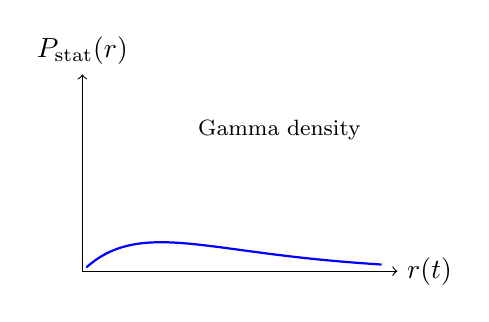
\begin{tikzpicture}
    \draw[->] (0,0) -- (4,0) node[right] {$r(t)$};
    \draw[->] (0,0) -- (0,2.5) node[above] {$P_{\mathrm{stat}}(r)$};
    \draw[thick, blue, domain=0.05:3.8, samples=80]
        plot (\x, {\x*exp(-\x)});
    \node[font=\footnotesize] at (2.5, 1.8) {Gamma density};
\end{tikzpicture}
\caption{An illustrative stationary CIR Gamma density, with shape $2$ and rate $1$ in scaled rate units.
These parameters describe a general CIR model, not the special squared-OU construction above.}
\label{fig:cir-chi2}
\end{figure}

Yet another route to positivity is the \emph{exponential Vasi\v{c}ek} model, obtained by modelling the \emph{logarithm} of the rate as an OU process:
\begin{equation}
Y(t) = \ln r(t) \quad\Longrightarrow\quad r(t) = \exp\{Y(t)\} > 0,
\end{equation}
so that $r$ is log-normal --- approximately what one sees in the data.

\subsection{Solution of the term structure equation}\label{sec:vasicek-term-structure}

We now return to the term structure equation~\eqref{eq:term-structure} and solve it with the OU specification.
Assuming constant $q$ and substituting $f = \alpha(\theta-r)$ and $S=\sigma$, the drift correction combines with the market price of risk into
\begin{equation}
f + S\,q = \alpha(\theta^* - r),
\qquad
\theta^* = \theta + \frac{\sigma\,q}{\alpha},
\end{equation}
% CLAUDE NOTE: θ* is the risk-adjusted long-run mean: θ shifted by the market price of risk.
so the whole effect of risk aversion is to shift the long-run mean from $\theta$ to the \emph{risk-adjusted} value $\theta^*$ --- an economical piece of bookkeeping.
The problem is then
\begin{equation}
\frac{\partial B}{\partial t} + \alpha(\theta^*-r)\,\frac{\partial B}{\partial r} + \frac{1}{2}\sigma^2\,\frac{\partial^2 B}{\partial r^2} = r\, B, \qquad B(T) = 1.
\end{equation}

The equation is linear in $r$ in its coefficients, which suggests an exponential-affine \emph{ansatz}:
\begin{equation}
P(r,t;T) = A(t,T)\, e^{-r\, B_0(t,T)},
\end{equation}
with terminal conditions $A(T,T) = 1$ and $B_0(T,T) = 0$ (so that $P(r,T;T)=1$ as required).
% CLAUDE NOTE: The notes use P for the trial solution and B₀ for the exponent coefficient
% to avoid confusion with the bond price B. We follow this convention.
The derivatives of the ansatz are
\begin{equation}
\partial_t P = \dot{A}\, e^{-rB_0} - r\dot{B}_0\, A\, e^{-rB_0},
\qquad
\partial_r P = -A\,B_0\,e^{-rB_0}, \qquad \partial^2_r P = A\,B_0^2\,e^{-rB_0},
\end{equation}
and substituting into the PDE and dividing through by $A\, e^{-rB_0}$,
\begin{equation}
\frac{\dot{A}}{A} - r\dot{B}_0 - \alpha(\theta^*-r)\,B_0 + \frac{1}{2}\sigma^2\,B_0^2 = r.
\end{equation}
Now comes the decisive observation: this must hold \emph{for every value of $r$}, and $r$ appears only linearly.
The coefficient of $r$ and the $r$-independent part must therefore vanish \emph{separately} --- the PDE splits into two ordinary differential equations.

Collecting the terms linear in $r$ (including the right-hand side),
\begin{equation*}
-\dot{B}_0 + \alpha B_0 - 1 = 0 \quad\Longrightarrow\quad \dot{B}_0 = \alpha B_0 - 1,
\qquad\text{(a)}
\end{equation*}
and collecting the constant terms,
\begin{equation*}
\frac{\dot{A}}{A} - \alpha\theta^*\,B_0 + \frac{1}{2}\sigma^2\,B_0^2 = 0.
\qquad\text{(b)}
\end{equation*}

Equation (a) is a linear first-order ODE.
Its general solution is $B_0(t,T) = Ce^{\alpha t} + \frac{1}{\alpha}$, and imposing $B_0(T,T)=0$ fixes $C = -\frac{1}{\alpha}\,e^{-\alpha T}$, whence
\begin{equation}\label{eq:vasicek-B}
B_0(t,T) = \frac{1}{\alpha}\bigl(1 - e^{-\alpha(T-t)}\bigr).
\end{equation}
Note the two limits: $B_0\approx T-t$ for short maturities (the bond behaves like $e^{-r(T-t)}$, as it must), while $B_0\to1/\alpha$ for long maturities --- mean reversion caps the sensitivity of long bonds to the current rate.

With $B_0$ known, equation (b) determines $A$ by separation of variables:
\begin{equation}
\frac{dA}{A} = \Bigl[\alpha\theta^*\,B_0 - \frac{1}{2}\sigma^2\,B_0^2\Bigr]dt,
\end{equation}
with $A(T,T) = 1$, i.e.\ $\ln A(T,T) = 0$.
Integrating from $t$ to $T$,
\begin{equation}
\ln A(t,T) = \int_t^T \bigl[-\alpha\theta^* B_0(s,T) + \tfrac12\sigma^2 B_0^2(s,T)\bigr]ds,
\end{equation}
and carrying out the (elementary if tedious) integrals yields
\begin{equation}\label{eq:vasicek-A}
\ln A(t,T) = \Bigl(\theta^* - \frac{\sigma^2}{2\alpha^2}\Bigr)\bigl[B_0(t,T) - (T-t)\bigr] - \frac{\sigma^2}{4\alpha}\,B_0^2(t,T),
\end{equation}
% CLAUDE NOTE: This is equivalent to the formula
% ln A = (θ* - σ²/2α²)[(1-e^{-α(T-t)})/α - (T-t)] - σ²/(4α) · [(1-e^{-α(T-t)})/α]²
which passes the sanity check $\ln A(T,T)=0$, since both $B_0(T,T)$ and $T-T$ vanish.

Assembling the pieces, the Vasi\v{c}ek bond price is
\begin{equation}
P(r,t;T) = A_{\text{Vas}}(t,T)\, e^{-r\,B_0(t,T)} =: P_{\text{Vas}}(r,t;T;\, \alpha, \theta^*, \sigma),
\end{equation}
an explicit closed formula --- the bond-market counterpart of the Black--Scholes formula.


\section{Calibration}\label{sec:vasicek-calibration}

A pricing formula is only useful once its parameters are pinned to the market, and the Vasi\v{c}ek model has three: $\alpha$, $\sigma$, and $\theta^*$.
The yield to maturity gives us the handle.
On the empirical side,
\begin{equation}
R(t,T) = -\frac{1}{T-t}\,\ln P(r,t;T) \quad\longrightarrow\quad \text{measured from quoted bond prices},
\end{equation}
while on the theoretical side the model predicts
\begin{equation}
R_v(r,t;T;\,\alpha,\theta^*,\sigma) = -\frac{1}{T-t}\,\ln P_v(r,t;T;\,\alpha,\theta^*,\sigma).
\end{equation}
The pricing mean $\theta^*$ must be inferred from market prices as well as historical dynamics.\footnote{The phrase ``tirato fuori dal mercato'' is a paraphrase in the handwritten lecture notes, not a verified quotation from Bj\"ork.
For the distinction between historical dynamics and pricing dynamics, see Bj\"ork\cite{Bjork2020}, the chapters on short-rate models.}


The calibration proceeds in two steps, each using the data best suited to it.
First, one fits $\alpha$ and $\sigma$ --- the dynamical parameters --- from the historical time series of the spot rate $r(t)$, by a best fit of the observed relaxation and fluctuations.
Second, one fits $\theta^*$ --- the risk-adjusted level, invisible in the history because it contains the market price of risk --- from today's \emph{yield curve}: at the observed maturities ($1, 2, 3, 4, 5, 10, 20$ years, \ldots) one imposes
\begin{equation}
R_{\text{emp}}(t,T) - R_{\text{the}}(r,t;T;\,\alpha,\sigma,\theta^*) = 0
\end{equation}
and fits $\theta^*$, generally by minimizing the discrepancies over maturities; one parameter need not match every quoted yield exactly.
Figure~\ref{fig:yield-curve} illustrates an upward-sloping model curve with synthetic observations; it is not an empirical calibration.

\begin{figure}[h!]
\centering
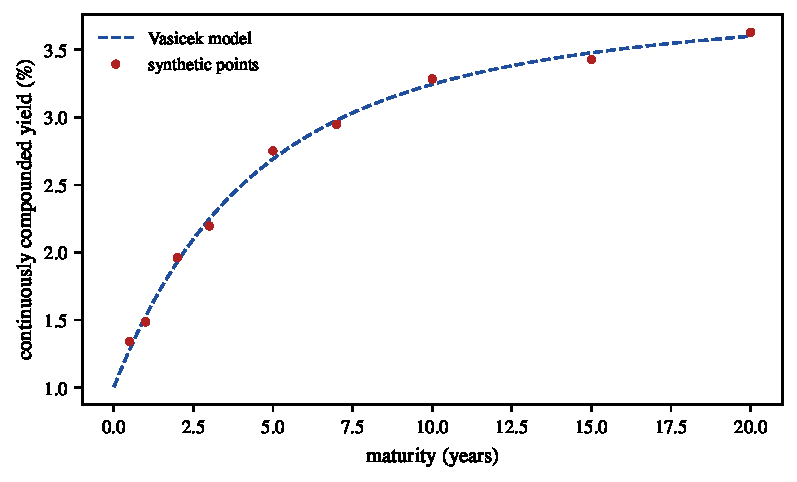
\includegraphics[width=0.72\textwidth]{images/vasicek_yield_review.pdf}
\caption{Illustrative Vasi\v{c}ek yield curve ($r=1\%$, $\alpha=0.4$, $\theta^*=4\%$, $\sigma=1\%$ in annual units), with synthetic perturbed points.
No market data were fitted.}
\label{fig:yield-curve}
\end{figure}

With all parameters fixed, the model prices not only the bonds themselves but the derivatives written on them: in the market one actively trades \emph{bond options}, whose valuation depends on exactly the parameters just calibrated.
The interplay between an analytically solvable model and a market calibration is the same we met for Black--Scholes --- and, as there, the model's Gaussian simplicity is both its strength and its limitation.
The next chapter confronts those limitations head-on.
